\section{Auswertung}
\label{sec:Auswertung}
\subsection{Statische Methode}

Mit Hilfe der geplotteten Graphen und der Temperaturmessung nach 700 Sekunden soll quantitativ die Wärmeleitfähigkeit der verschieden Proben bestimmt werden. In den Plots sind die Temperaturverläufe der Thermoelemente die am weitesten von dem Peltier Element entfernt sind zu sehen.
\begin{figure}
	\caption{Temperaturverlauf}
	\centering
	\begin{subfigure}{0.48\textwidth}
		\centering
  		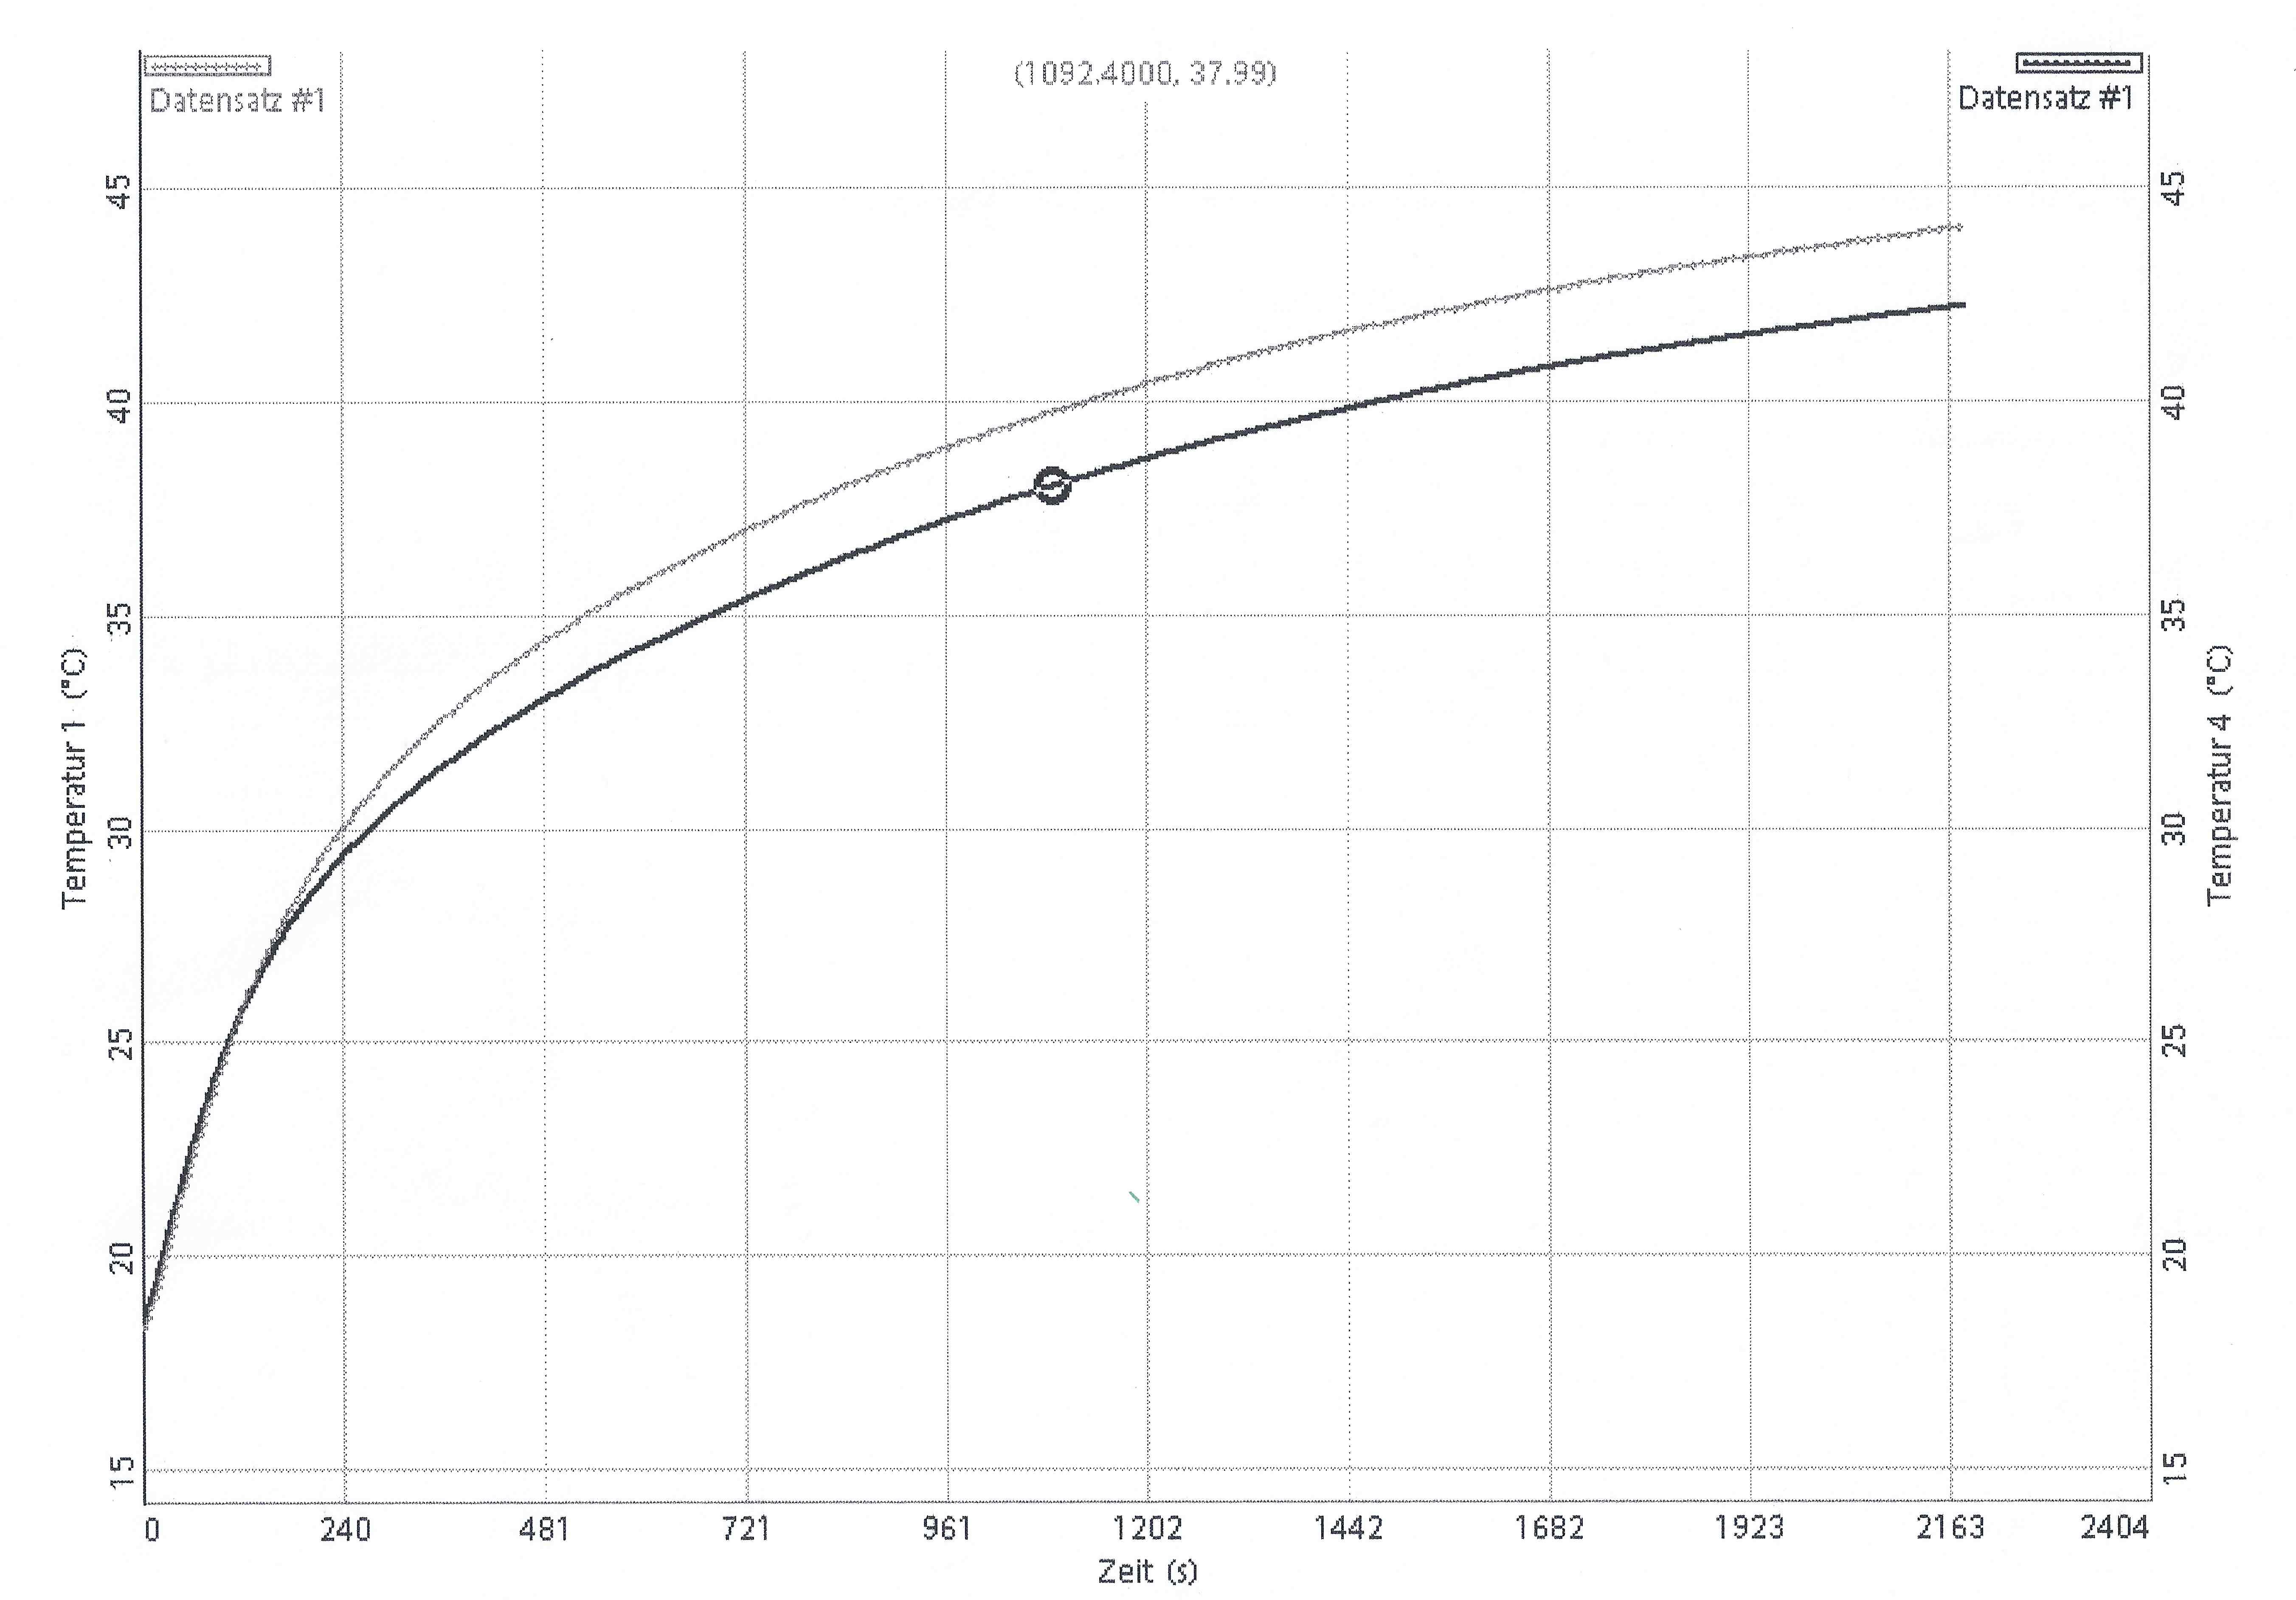
\includegraphics[height=4.5cm]{./Graph_4.png}
  		\caption{breiter (Temperatur 1) und schmaler (Temperatur 4) Messingstab}
		\label{fig:T1T4}
	\end{subfigure}
	\begin{subfigure}{0.48\textwidth}
  		\centering
  		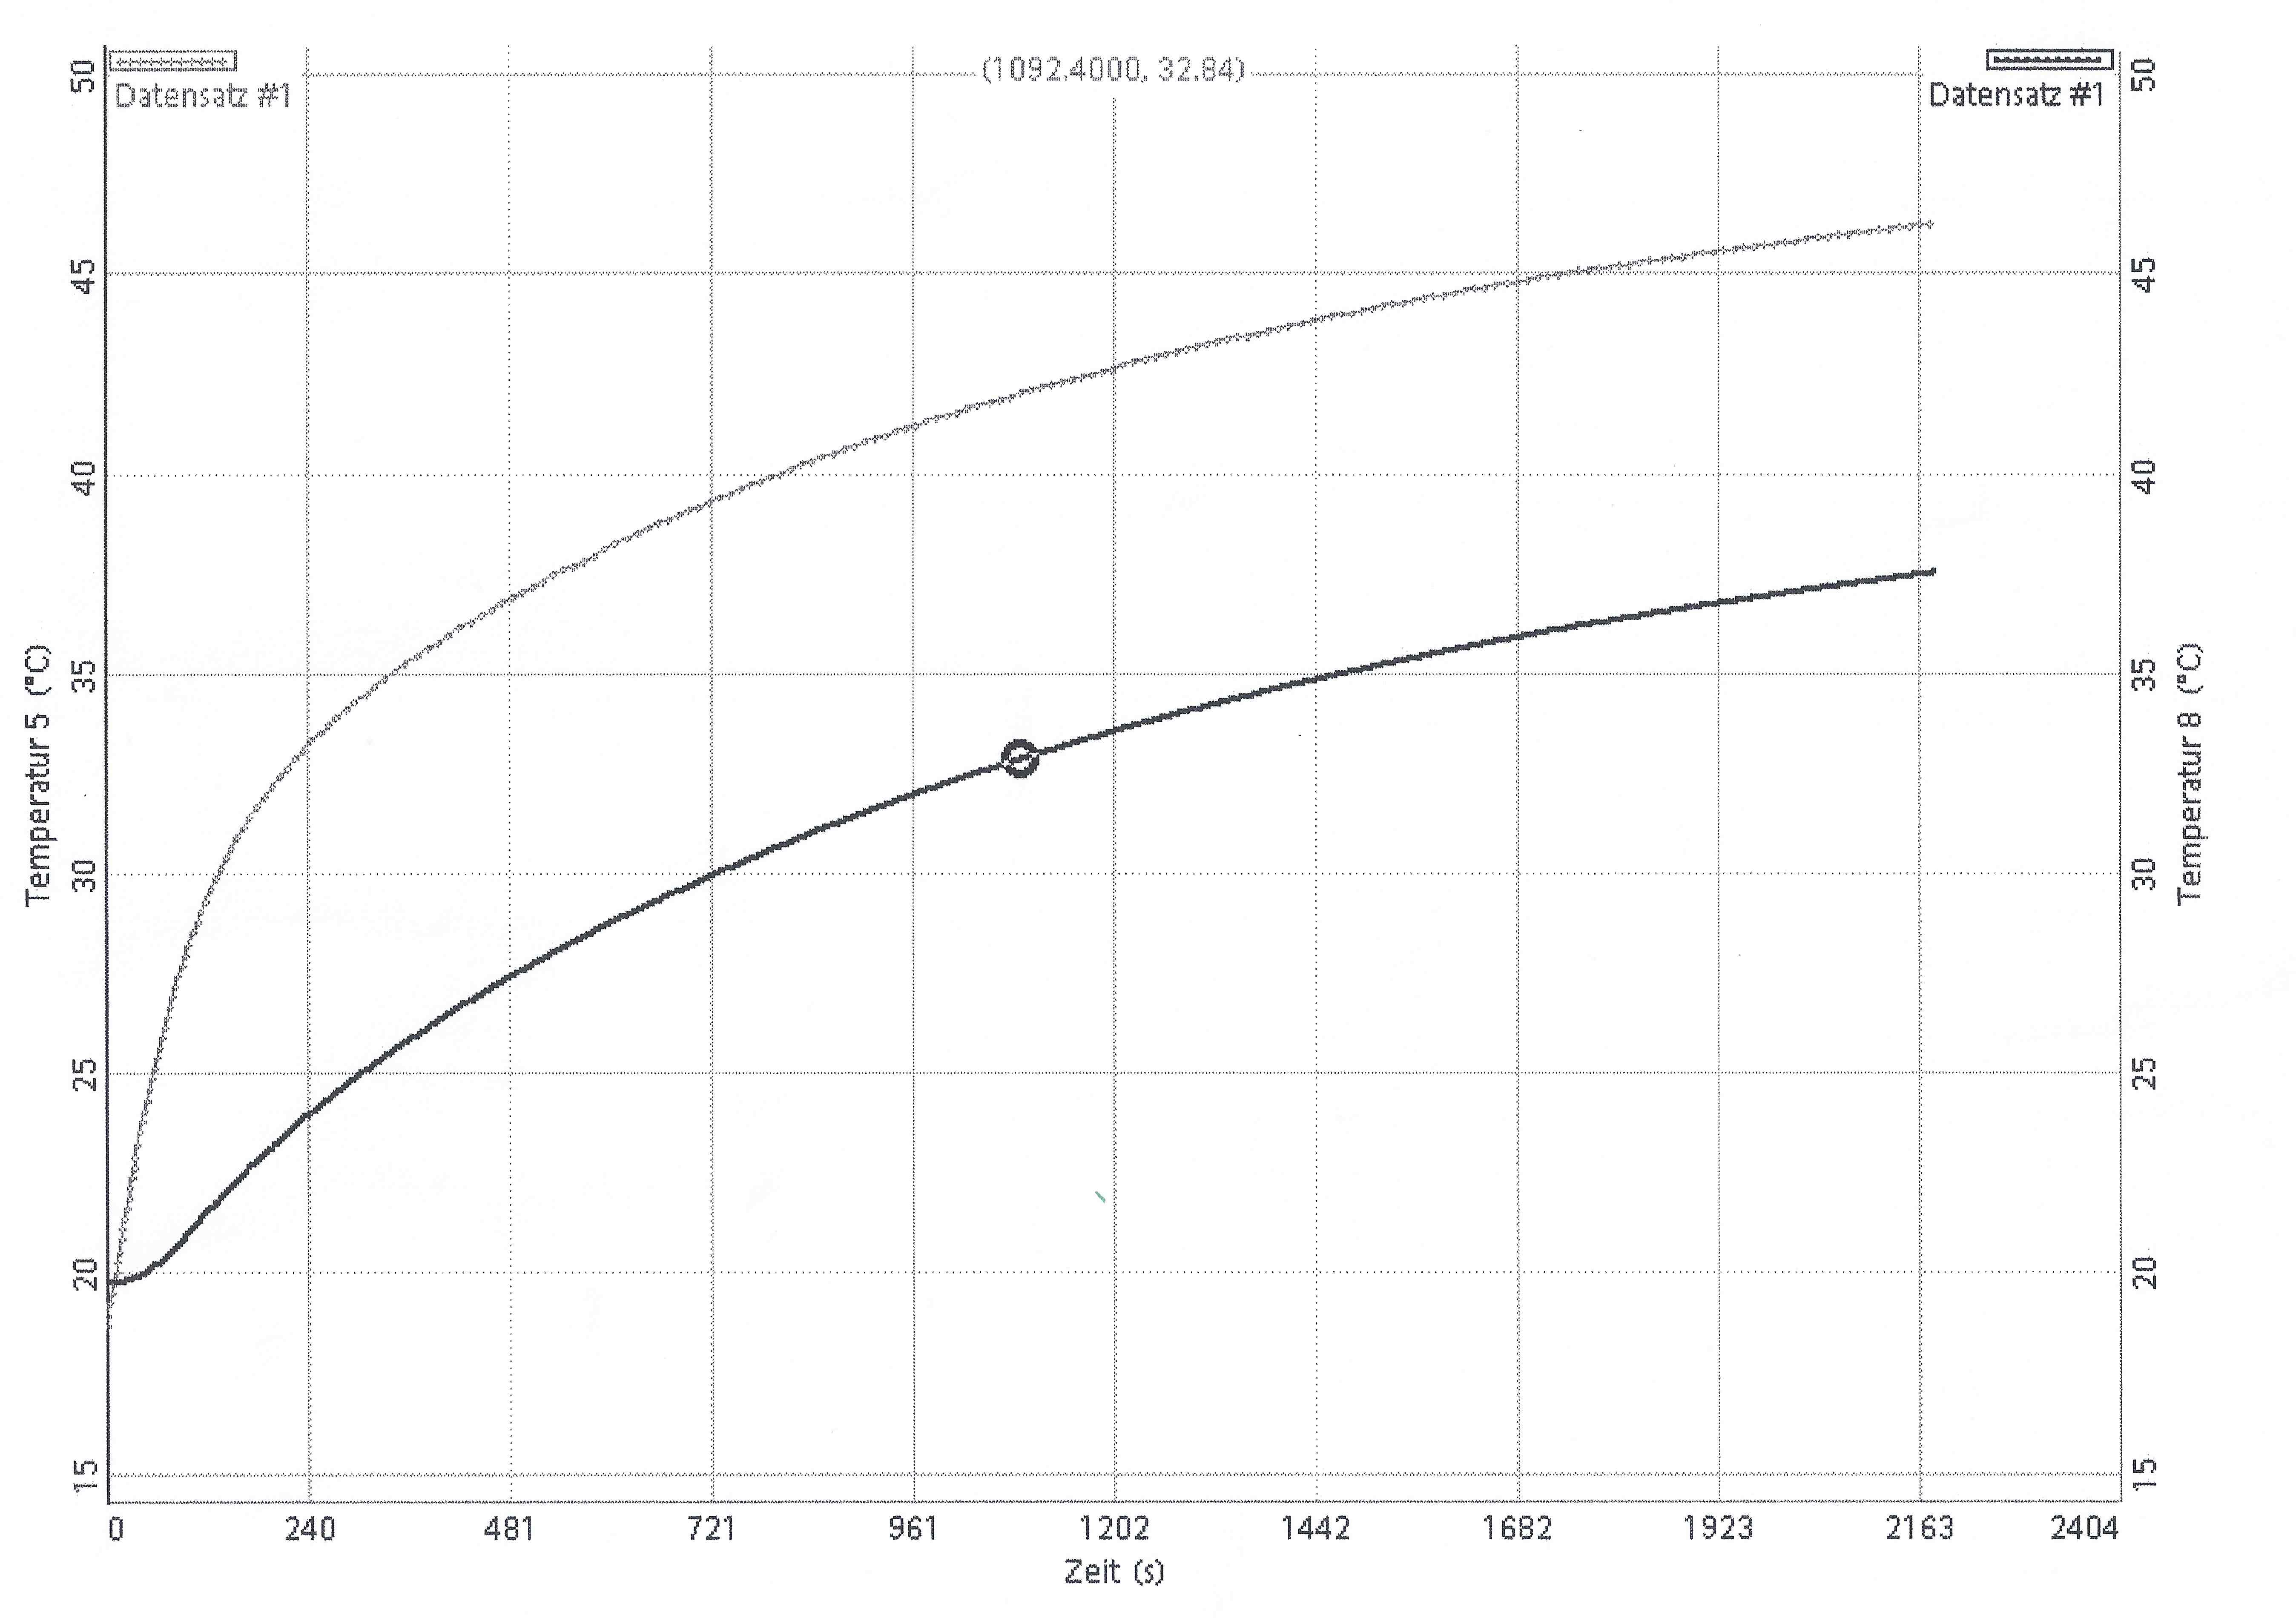
\includegraphics[height=4.5cm]{./Graph_5.png}
  		\caption{Aluminium (Temperatur 5) und Edelstahl (Temperatur 8)}
		\label{fig:T5T8}
	\end{subfigure}
\end{figure}
Auffällig ist das alle Graphen exponentiell ansteigen und nach einer bestimmten Zeit gegen unterschiedliche Sättigungswerte streben. Dabei ist der größte Anstieg in den ersten 240 Sekunden zu verzeichnen. Mit Hilfe der Ergebnisse der Temperaturmessung nach 700 Sekunden (siehe Tabelle \ref{tab:kelv}) und der Steigung der Graphen lassen sich Rückschlüsse auf die Wärmeleitfähigkeit ziehen. Da die Steigung des Graphen für Aluminium am größten ist und die Temperatur am meisten angesteigt, lässt sich daraus schließen das Aluminium die größte Wärmeleitfähigkeit $\kappa$ besitzt.
\begin{table}
	\centering
	\caption{Temperatur nach 700 Sekunden}
	\label{tab:kelv}
	\begin{tabular}{c}
		\toprule
		T [K] \\
		\midrule
		$T_1$ = 309.65 K \ \\
		$T_4$ = 308.03 K \ \\
		$T_5$ = 311.99 K \ \\
		$T_8$ = 302.59 K \ \\
		\bottomrule
	\end{tabular}
\end{table}
Um den Wärmestrom von Messing zu berechnen, wird  $T_2 - T_1$ für den breiten Messingstab und $T_7 - T_8$ für den Edelstahlstab in einem Diagramm aufgetragen.\ 
\begin{figure}
	\centering
	\caption{Temperaturdifferenz}
	\begin{subfigure}{0.48\textwidth}
		\centering
		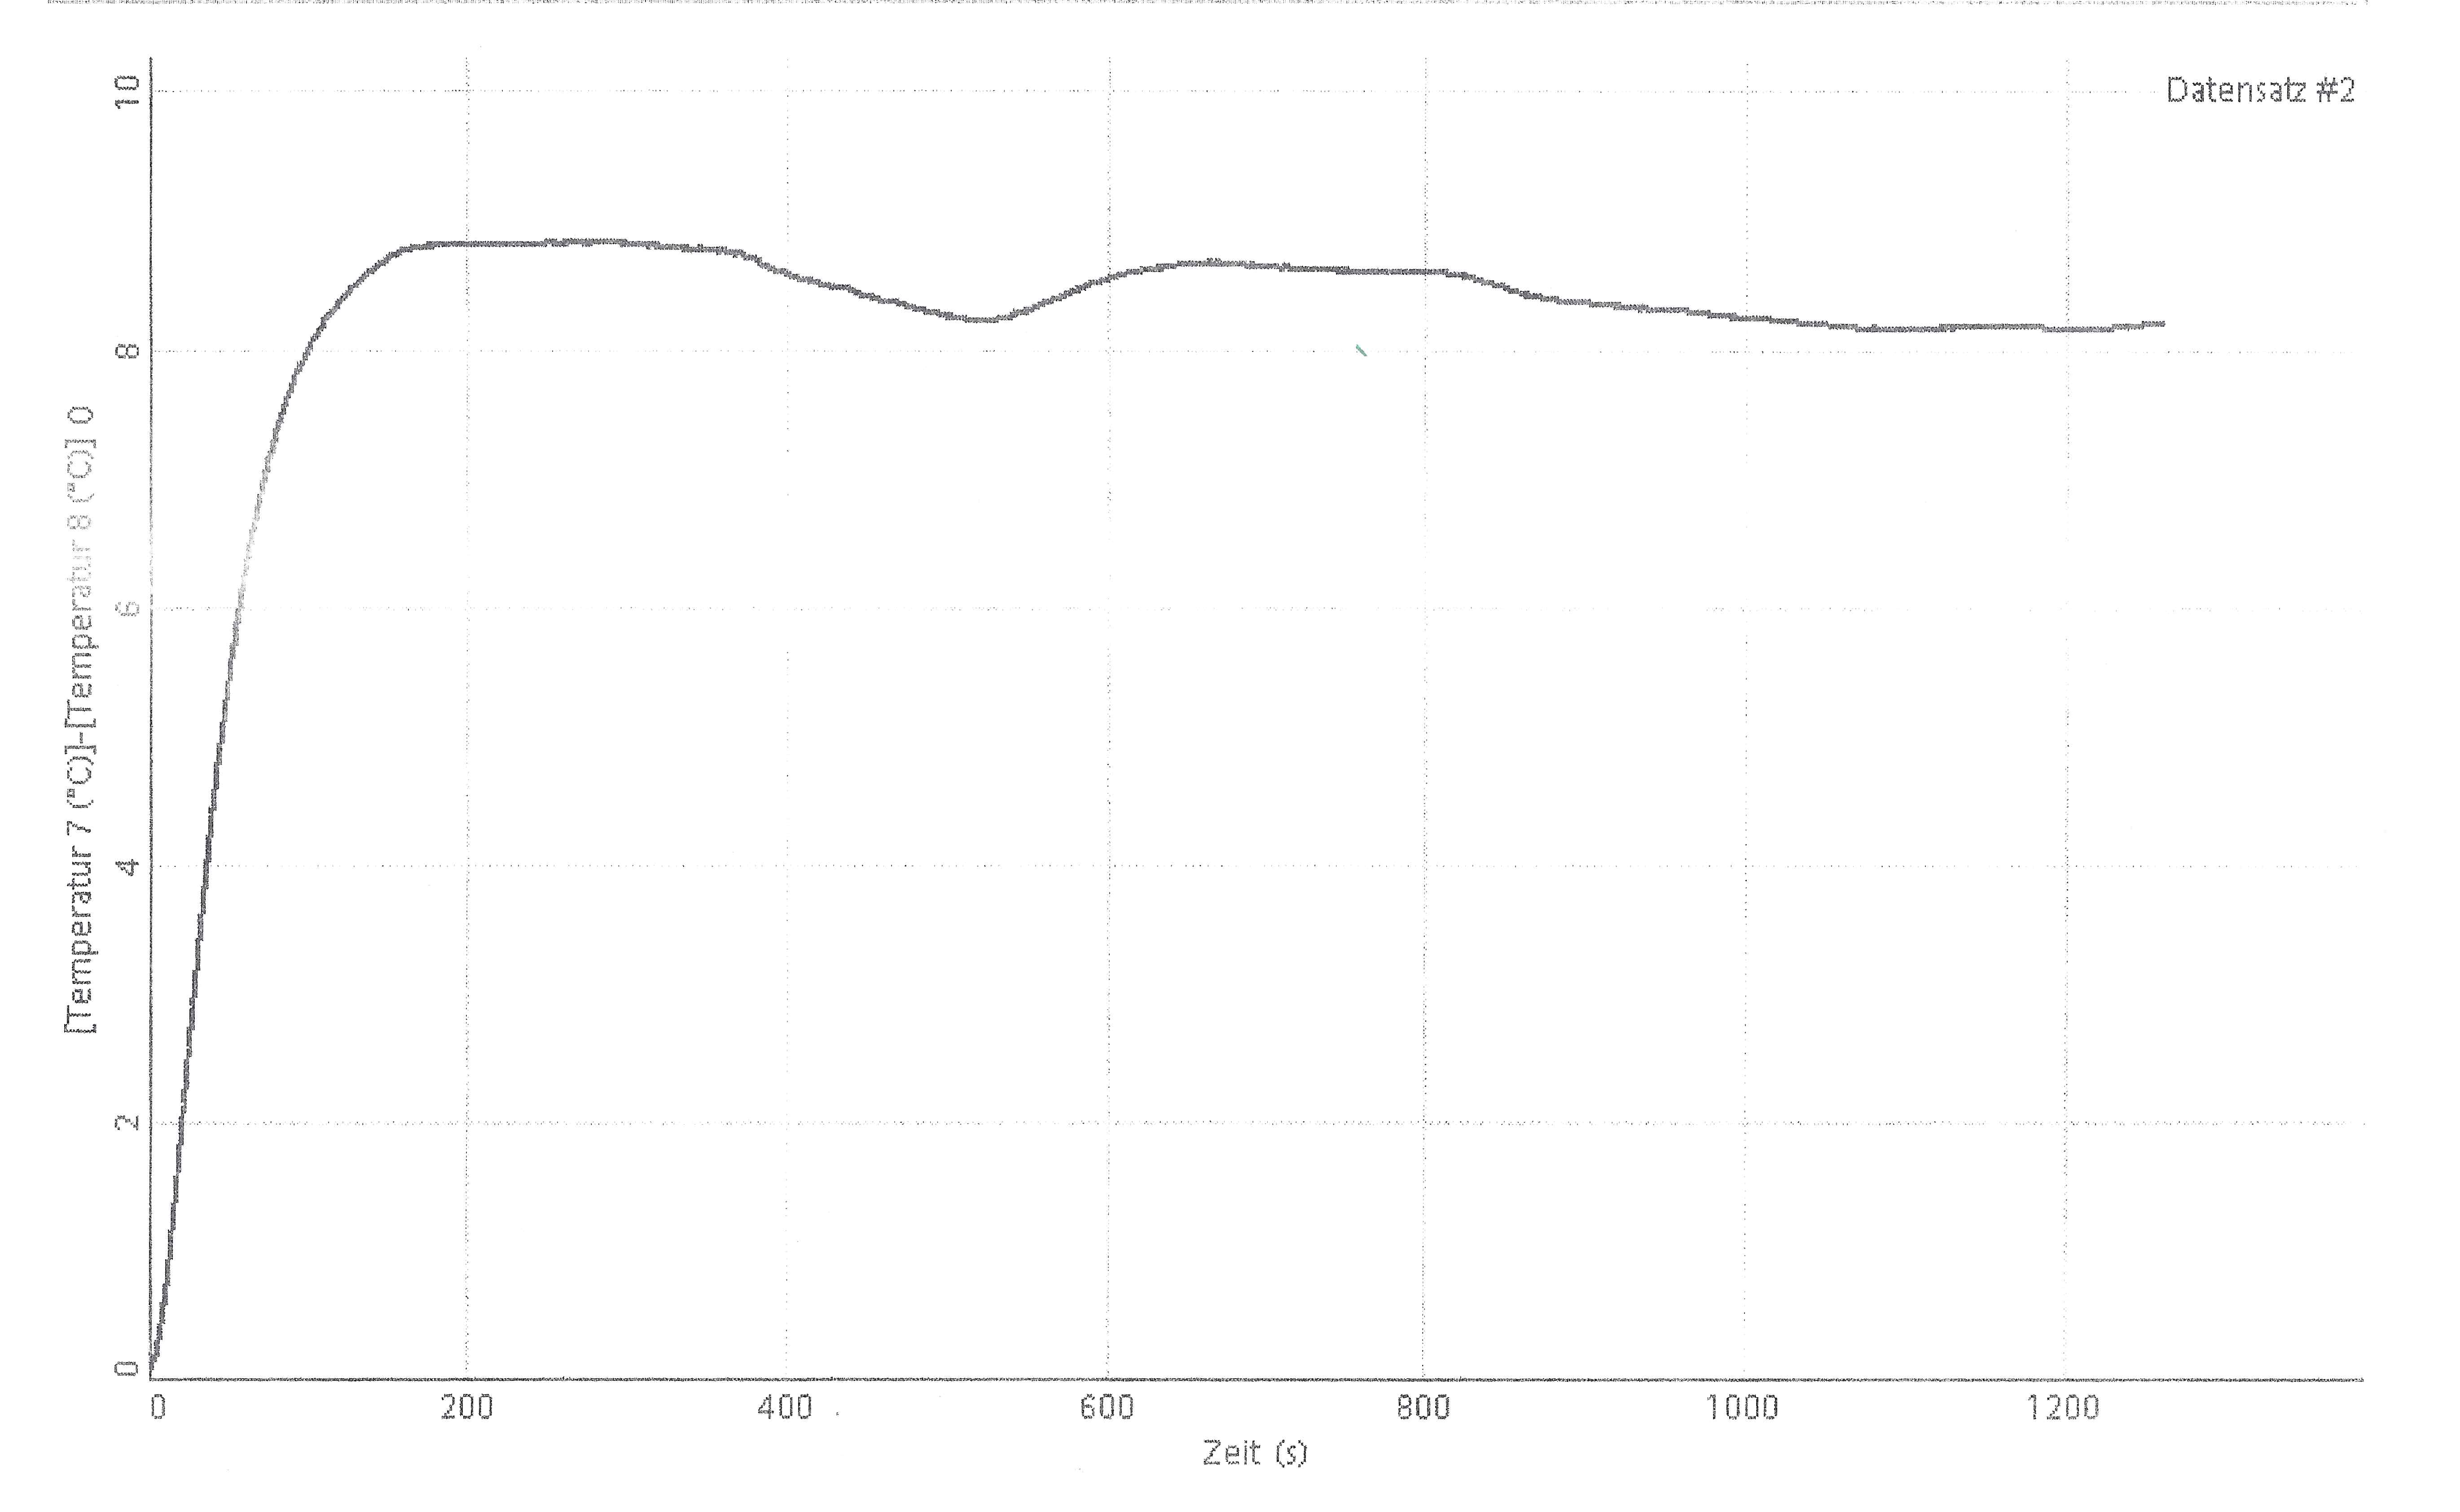
\includegraphics[height=4.5cm]{./Graph_6.png}
		\caption{Edelstahlstab}
	\end{subfigure}
	\begin{subfigure}{0.48\textwidth}
		\centering
                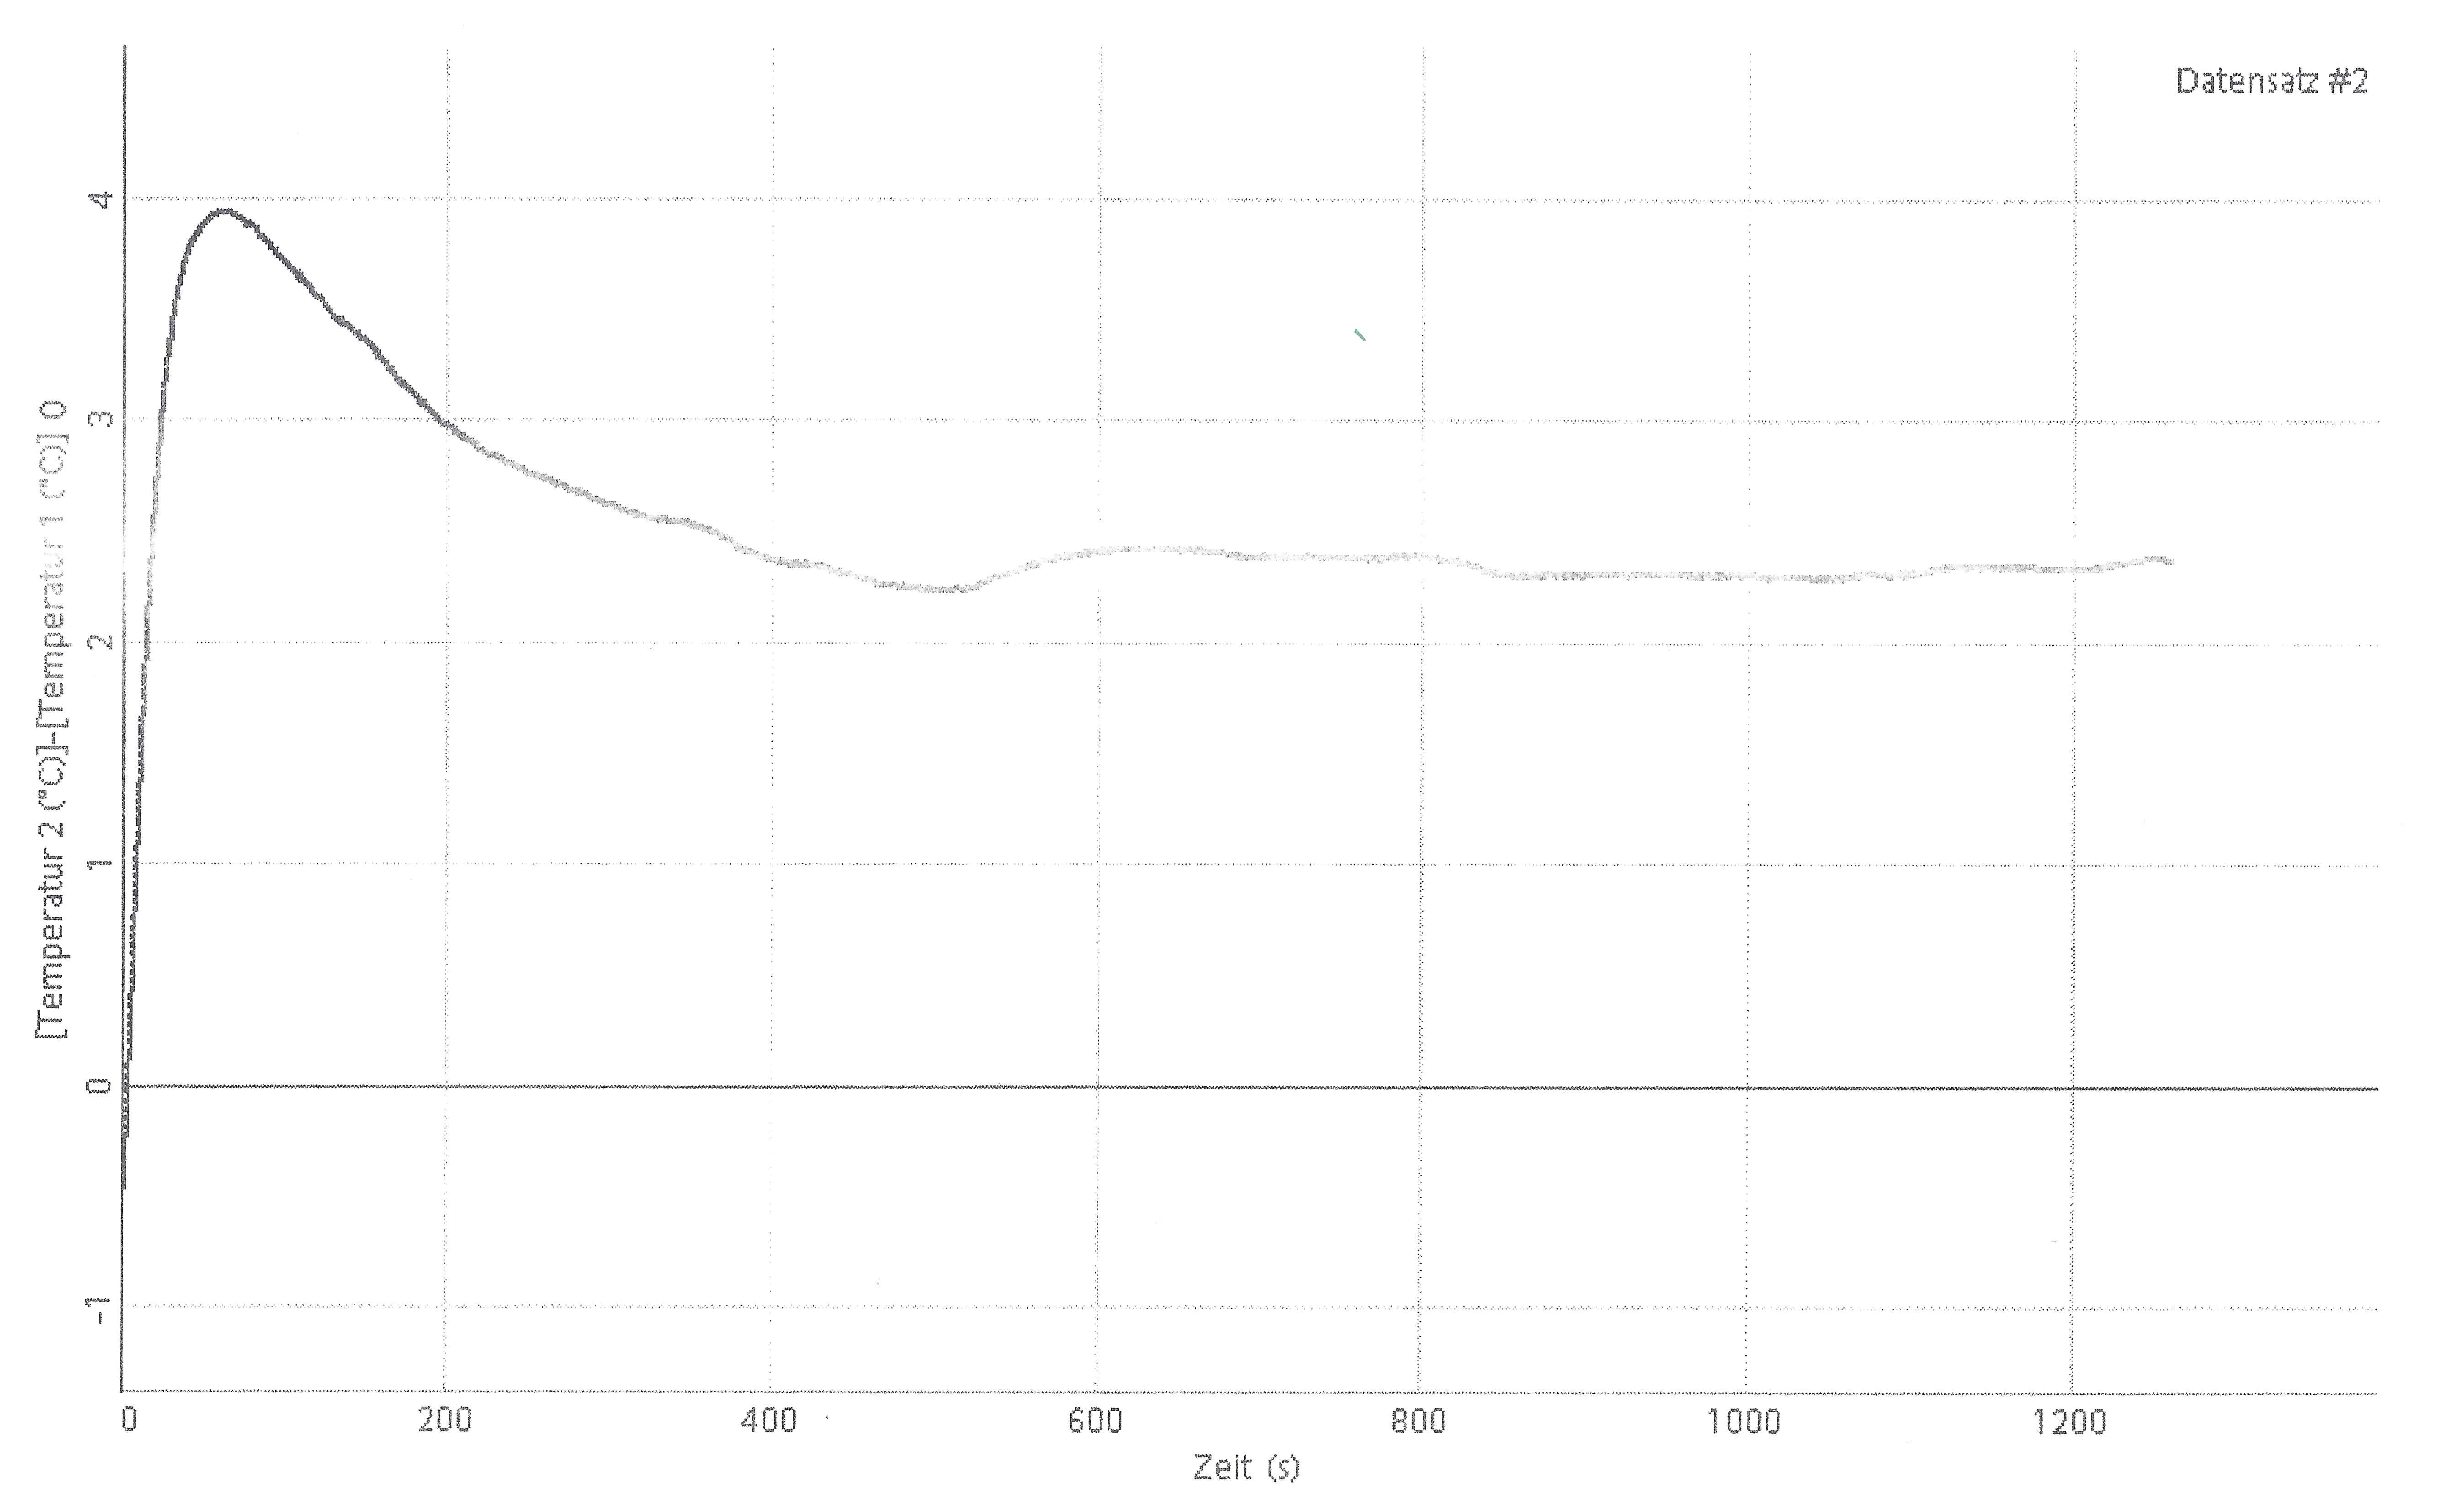
\includegraphics[height=4.5cm]{./Graph_7.png}
                \caption{breiter Messingstab}
        \end{subfigure}
\end{figure}
Beide Graphen steigen zu beginn in etwa gleich schnell an. Der Edelstahlstab erreicht nach fast 200 Sekunden seinen Grenzwert von 8 Kelvin. Der Messingstab hat nach ca. 50 Sekunden einen Peak und flacht danach gegen seinen Grenzwert von ca. 2.4 Kelvin ab. Der Peak lässt sich dadurch erklären, dass das an dem Peltier Element nahe Thermoelement schon von dem Wärmestrom erhitzt wird und das ferne Thermoelemt noch nicht.
Die Wärmemenge pro Zeit lässt sich durch division der Gleichung \ref{eqn:Q/t} durch $dt$ berechnen. Dafür wurde der Wert $\kappa$ aus der Literatur entnommen und der Querschnitt der Versuchsanleitung entnommen.
\begin{eqnarray*} 
		 \kappa_{Messing} 	& =& 120 \frac{\text{W}}{\text{m K}}  		\\
		 A_{Messing} 		& =& 4.8 \cdot 10^{-5} \text{m}^2		\\
		 \Delta x_{Messing}	& =& 0.03 \, \text{m}				\\
		 \kappa_{Edelstahl}	& =& 15\frac{\text{W}}{\text{m K}}      	\\
                 A_{Edelstahl}          & =& 4.8 \cdot 10^{-5}\text{m}^2           	\\
                 \Delta x_{Edelstahl}   & =& 0.03 \, \text{m}           		\\
\end{eqnarray*}
Die Messergebnisse des Wärmestrom pro Zeit wurden in Tabelle \ref{tab:wärmestrom} für die verschieden Zeiten berechnet.
\begin{table}
	\centering
	\caption{Temperaturdifferenz des breiten Messingstabes ($T_2 - T_1$) und des Edelstahlstabes ($T_7 - T_8$)}
	\label{tab:wärmestrom}
	\begin{tabular}{c c c c c}
		\toprule
		Messzeit [s] & ($T_2 - T_1$) [K] & $ \frac{\Delta Q_{21}}{\Delta t}$ [W] & $(T_7 - T_8)$ [K] & $ \frac{\Delta Q_{78}}{\Delta t}$ [W] \\
		\midrule
		200  & 3.0	& -0.5760 & 8.8	&-0.2112	\\
		400  & 2.4	& -0.4608 & 8.6	&-0.2064	\\
		600  & 2.4	& -0.4608 & 8.6	&-0.2064	\\
		800  & 2.4	& -0.4608 & 8.6	&-0.2064	\\
		1000 & 2.3	& -0.4416 & 8.4	&-0.2016	\\
		\bottomrule
	\end{tabular}
\end{table}

\subsection{Dynamische Methode}
\subsubsection{Aluminium und Messing}
Mit hilfe periodischem Heizen soll nun die Materialkonstante $\kappa$ bestimmt werden. Die beiden graphischen Verläufe beider Thermoelemente sind in Diagramm \ref{fig:Tdiff} \subref{fig:Graph1} und \subref{fig:Graph2} zu sehen. Durch bestimmung des Amplitudenverhältnisses $A_{nah}$ und $A_{fern}$ und der Phasendifferenz $\Delta t$ lässt sich durch einsetzen in Gleichung \ref{eqn:kappa} die Materialkonstante $\kappa$ bestimmen. 
\begin{figure}
        \centering
        \caption{Temperatur der Thermoelemente bei periodischem Heizem}
        \label{fig:Tdiff}
	\begin{subfigure}{0.48\textwidth}
                \centering
                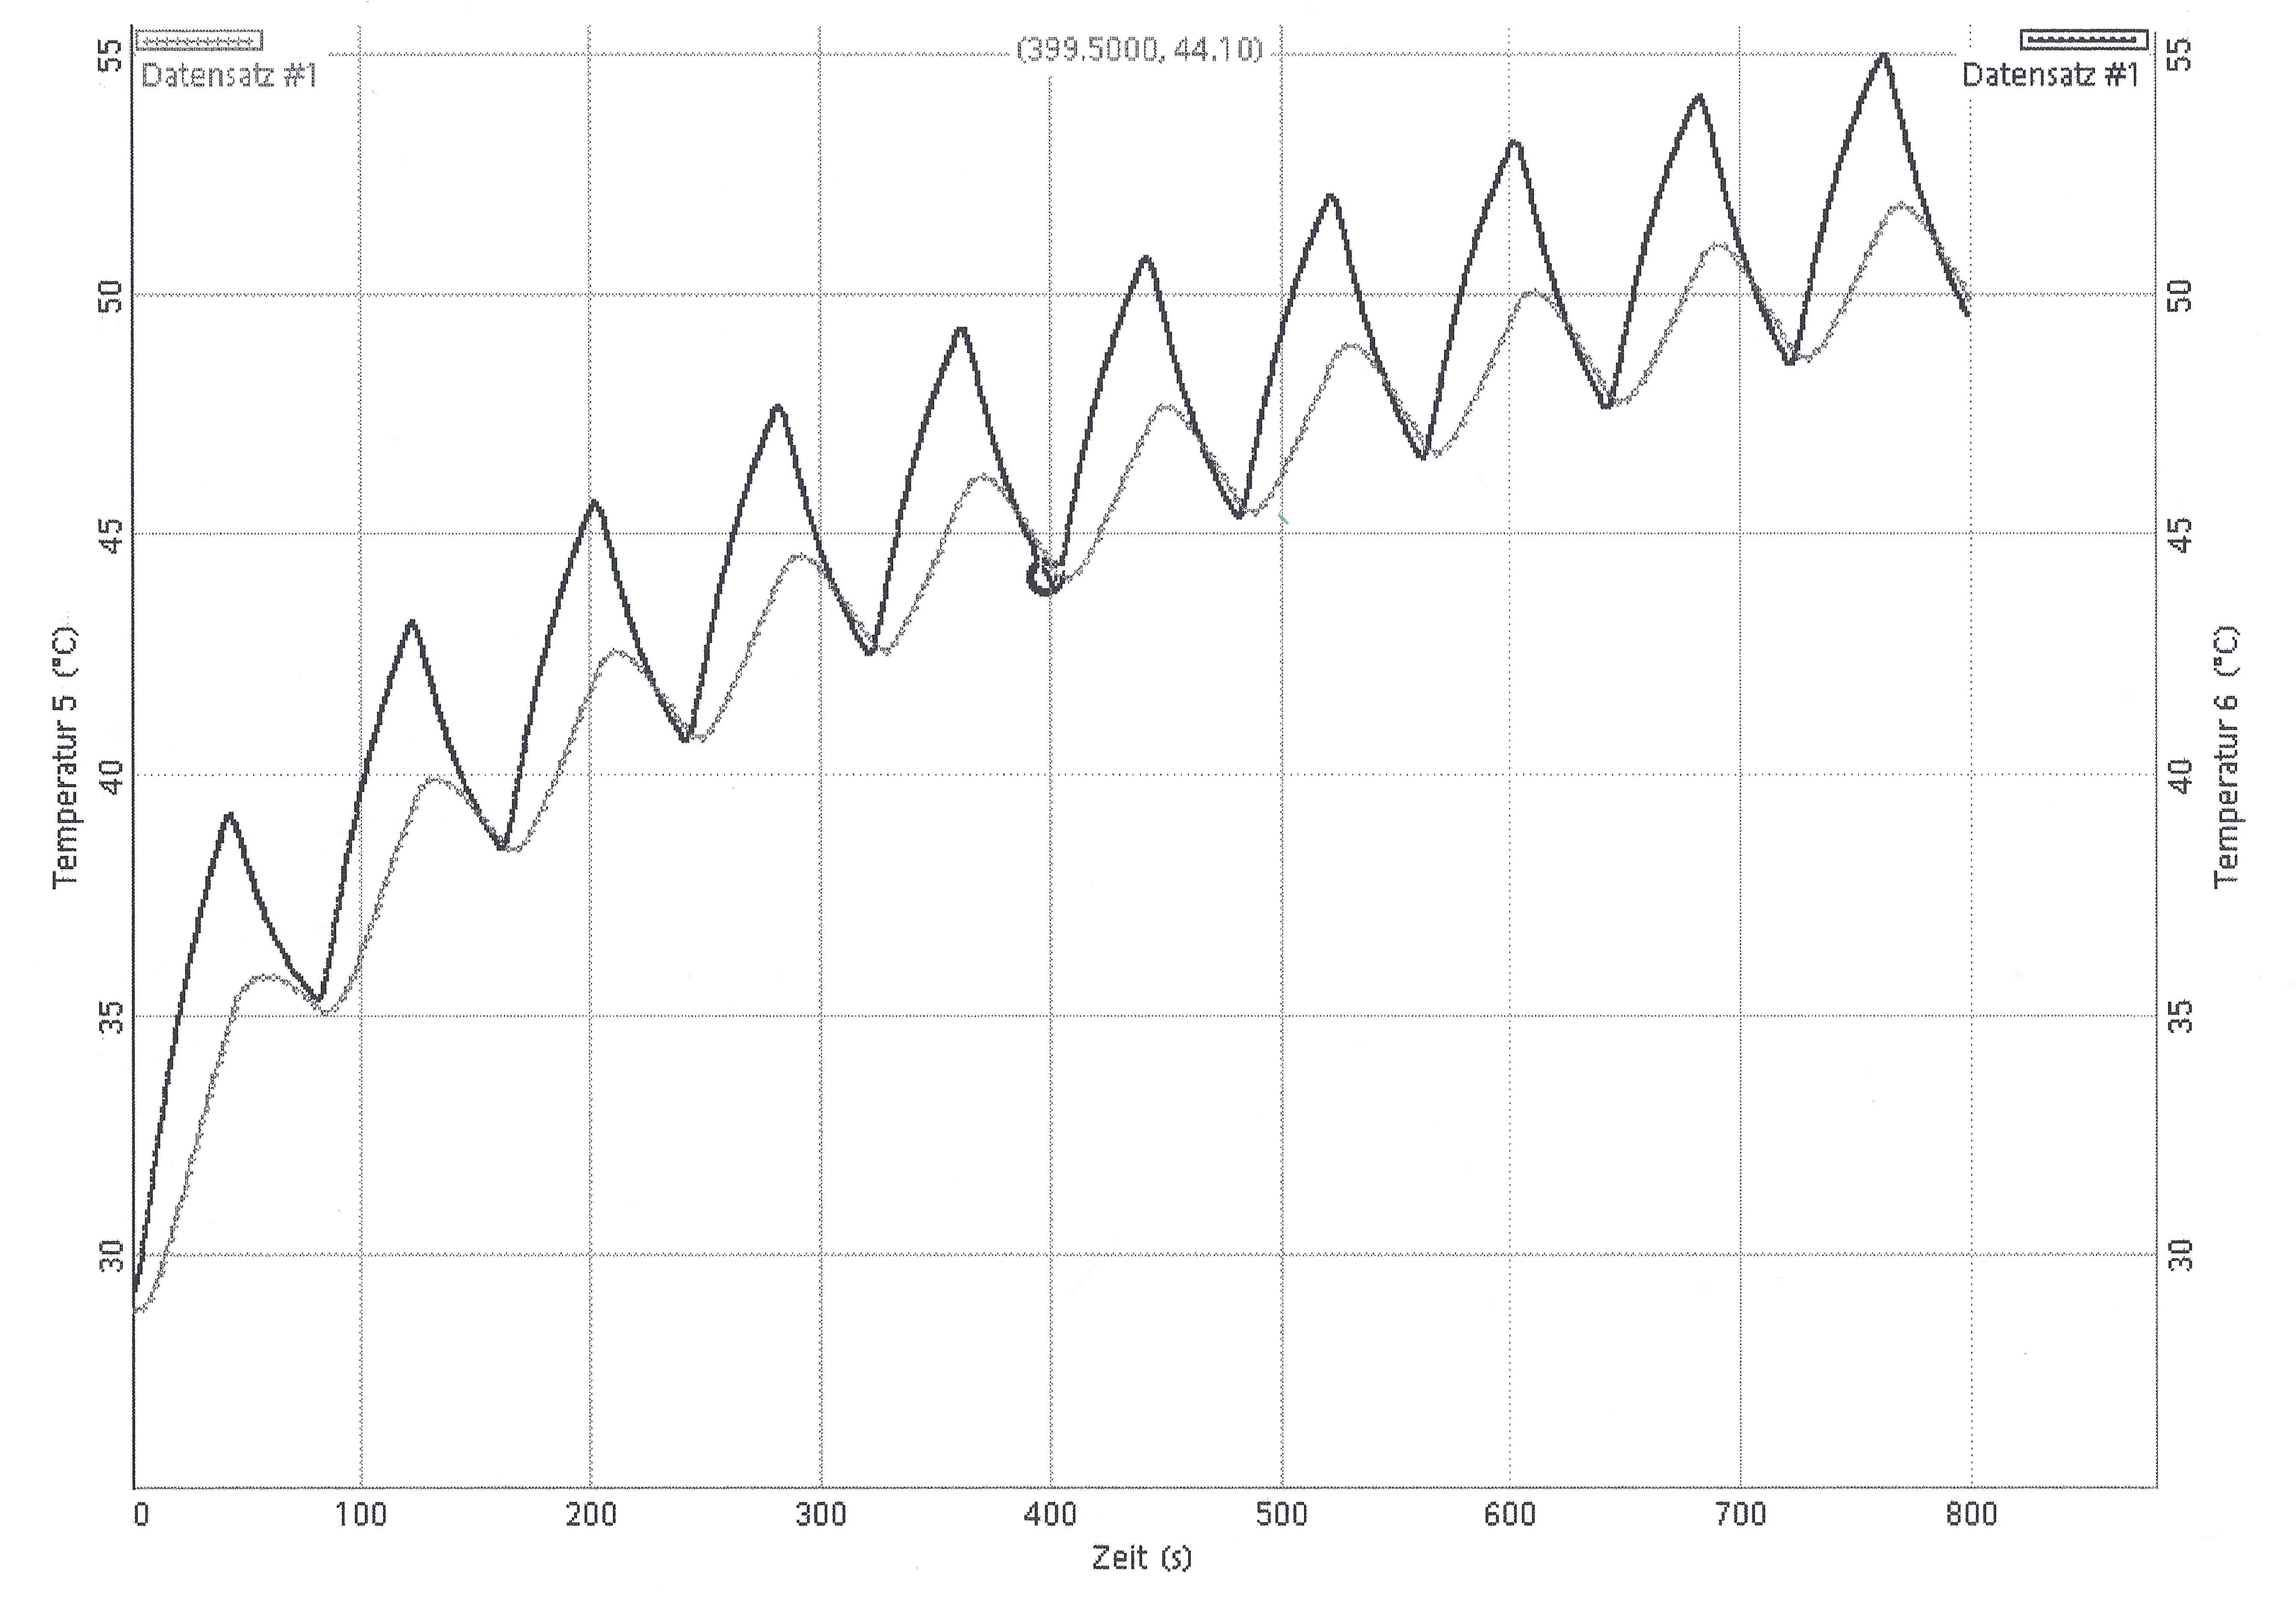
\includegraphics[height=4.5cm]{./Graph_1.png}
                \caption{Aluminium}
		\label{fig:Graph1}
        \end{subfigure}
        \begin{subfigure}{0.48\textwidth}
                \centering
                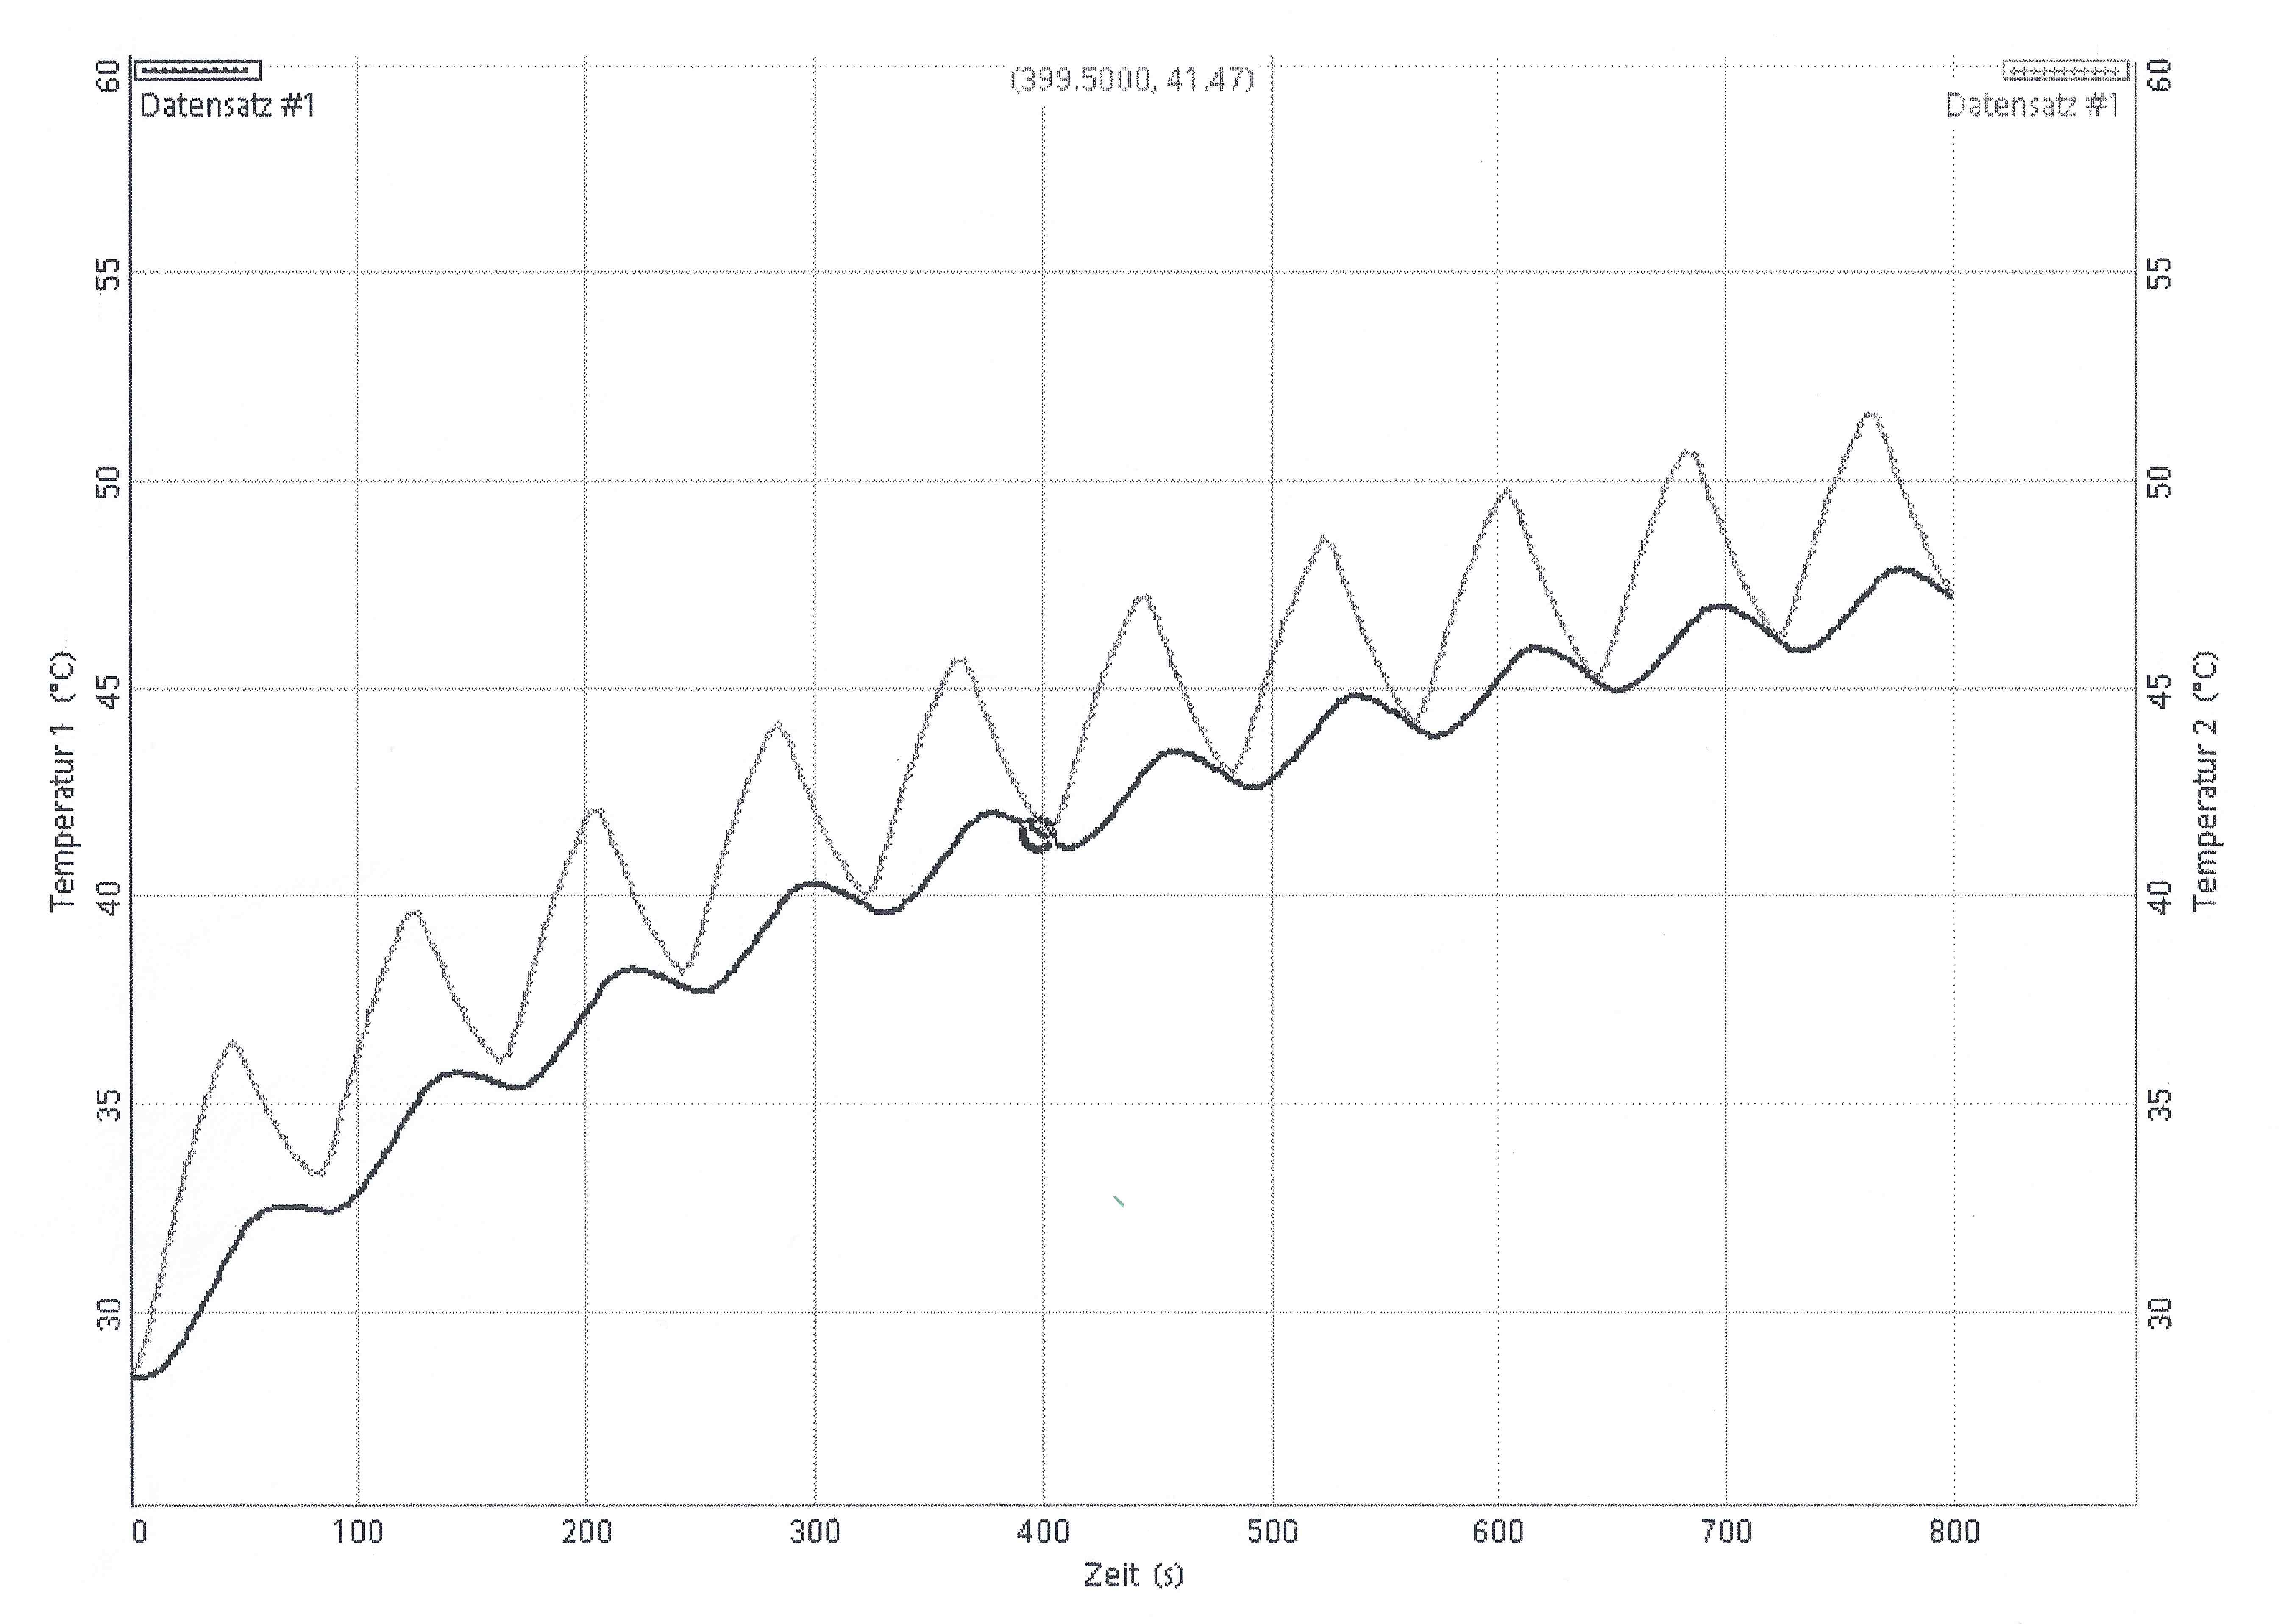
\includegraphics[height=4.5cm]{./Graph_2.png}
                \caption{breiter Messingstab}
		\label{fig:Graph2}
        \end{subfigure}
\end{figure}
Für Aluminium und Messing sind in Tabelle \ref{tab:AuP} deren Amplituden, Amplitudenverhältnisse sowie Phasendifferenz bei einer Periodendauer von 80 Sekunden aufgeführt. 
\begin{table}
	\centering
	\caption{Amplitudenverhältnisse und Phasendifferenz}
	\label{tab:AuP}
	\begin{tabular}{c c c c c c c c}
		\toprule
		\multicolumn{4}{c}{Aluminium} & \multicolumn{4}{c}{Messing}\\
		$A_{nah}$ [K] & $A_{fern}$ [K] & $10^{-1}$ ln $ \left(\frac{A_{nah}}{A_{fern}} \right)$ & $\Delta t$ & $A_{nah}$ [K] & $A_{fern}$ [K] & ln $ \left( \frac{A_{nah}}{A_{fern}} \right) $& $\Delta t$ \\
		\midrule
		2.86 & 3.10 & -0.8 & 8  & 6.66 & 3.54 & 0.63 & 4 \\
		5.00 & 2.62 &  6.4 & 8  & 7.07 & 2.91 & 0.89 & 4 \\
		4.52 & 2.38 &  6.4 & 8  & 6.86 & 2.70 & 0.93 & 8 \\ 
		4.52 & 2.14 &  7.5 & 8  & 6.45 & 2.29 & 1.04 & 8 \\
		4.28 & 2.14 &  6.9 & 8  & 6.66 & 2.29 & 1.07 & 8 \\
		4.28 & 2.14 &  6.9 & 13 & 6.45 & 2.29 & 1.04 & 8 \\
		4.05 & 2.14 &  6.4 & 13 & 6.45 & 2.08 & 1.31 & 8 \\
		4.05 & 1.90 &  7.5 & 13 & 6.24 & 2.08 & 1.10 & 4 \\
		4.05 & 1.90 &  7.5 & 13 & 6.24 & 2.08 & 1.10 & 8 \\ 
		3.81 & 1.94 &  6.9 & 17 & 6.24 & 2.08 & 1.10 & 8 \\
		\bottomrule
	\end{tabular}
\end{table}		
In dem Versuschsaufbau wird durch Mittelung (siehe Formel \ref{eqn:Mittelwert} und \ref{eqn:Mittelwert_err}  der Messwerte die Wärmeleitung \kappa bestimmt.
\begin{eqnarray*}
	\Delta x 			=& ( \num{3.0 +- 0.1} ) \text{cm}	\\
	\Delta t_{Aluminium} 		=& ( \num{6.8 +- 1.8} ) \text{s}	\\
	\Delta t_{Messing}		=& ( \num{10.9 +- 3.1} ) \text{s}	\\
	\rho_{Aluminium}		=& 2800 \frac{\text{kg}}{\text{m}^3}			\\
	\rho_{Messing}			=& 8520 \frac{\text{kg}}{\text{m}^3}			\\
	c_{Aluminium}			=& 830 \frac{\text{J}}{\text{kg $\cdot$ K}}		\\
	c_{Messing}			=& 385 \frac{\text{J}}{\text{kg $\cdot$ K}}		\\
\end{eqnarray*}
Die Phasenverschiebung wird durch Messung des Abstands der Wellentiefpunkte der beiden Amplituden ermittelt. Die Werte für die Dichte als auch Spezifischer Wärmekapazität wurden dem Versuchsanleitung entnommen. 
Es ergibt sich eine Wärmeleitfähigkeit für Aluminium von 
\begin{equation}
	\kappa_{Aluminium} = (\num{160 +- 80}) \frac{\text{W}}{\text{m K}} \ ,
\end{equation}
und für Messing 
\begin{equation}
        \kappa_{Messing} = (\num{150 +- 50}) \frac{\text{W}}{\text{m K}} \ ,
\end{equation}

\subsubsection{Edelstahl}
Die Bestimmung der Wärmeleitfähigkeit von Edelstahl ist nicht möglich da sich am weiter entfernten Thermoelement keine Amplituden der Schwingung auf dem Graphen \ref{fig:Graph3} mehr zu erkennen sind. Somit lässt sich keine Phasenverschiebung als auch Amplitudenverhältniss mehr errechnen. 
\begin{figure}
        \centering
        \caption{Temperatur von Edelstahl bei periodischem Heizem}
        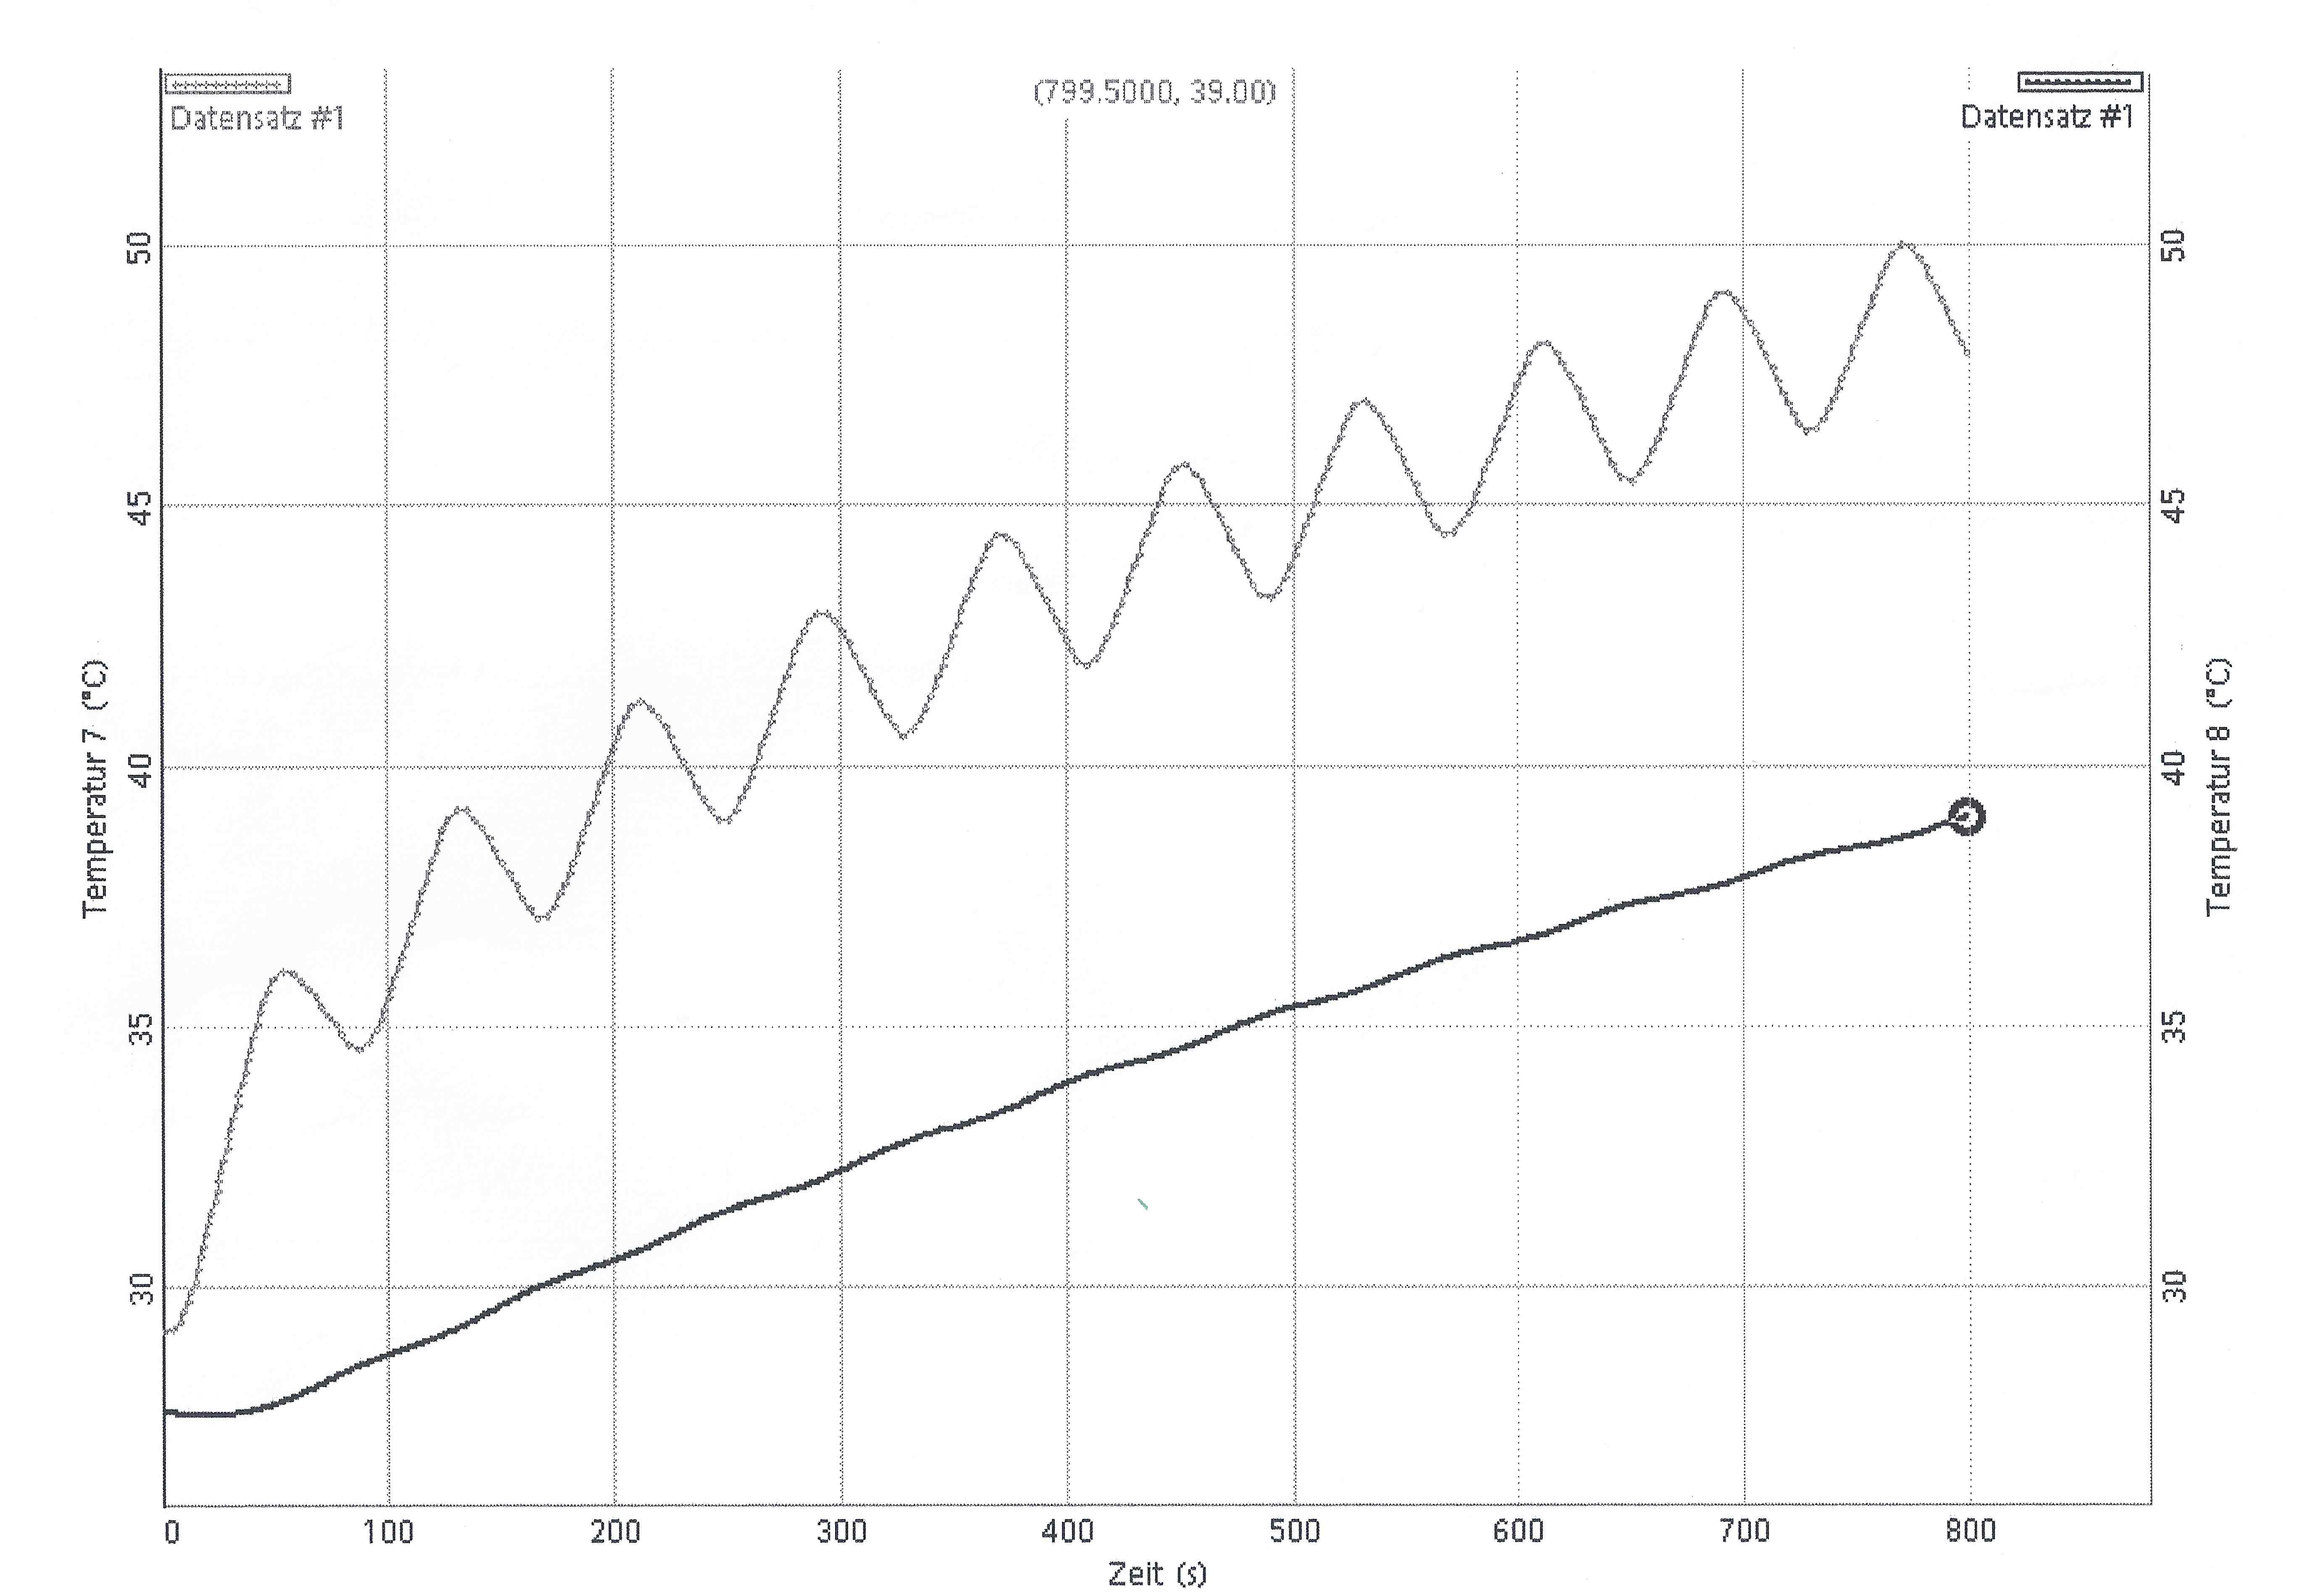
\includegraphics[height=4.5cm]{./Graph_3.png}
        \label{fig:Graph3}
\end{figure}

\subsection{Frequenz und Wellenlänge}
Die Frequenz der Wellen erhält ist der Kehrwert der Heizungsperioden. Somit beträgt die Frequenz 
\begin{equation}
	f = 0.013 \frac{1}{s} \ .  
\end{equation}
Um die Ausbreitungsgeschwindigkeiten der verschiedenen Stoffe zu berechnen werden die zuvor errrechneten Werte von $\kappa$ in Formel \ref{eqn:v} eingesetzt und es ergeben sich Geschwindigkeiten von 
\begin{equation}
	v_{Aluminium} =(\num{3.5 +- 7.0}) \cdot 10^{-3} \frac{\text{m}}{\text{s}}
\end{equation} 
und 
\begin{equation}
	v_{Messing} = (\num{2.8 +- 8.4}) \cdot 10^{-3} \frac{\text{m}}{\text{s}} 
\end{equation}
Aus den Ergebnissen ergibt sich aus der Beziehung 
\begin{equation}
	c = \lambda \cdot f
\end{equation} 
eine Wellenlänge von Aluminium von
\begin{equation}
        \lambda_{Aluminium} = (\num{0.0035 +- 0.007}) \text{m}
\end{equation}
und für Messing 
\begin{equation}
	\lambda_{Messing} = (\num{0.002 +- 0.006}) \text{m}
\end{equation}
